\documentclass[writeup.tex]{subfiles}
\begin{document}

\section{Part 3: A Fresh-Baked Holiday Pi} \label{section.part3}
	Before beginning on these quests, I needed to assemble the Cranberry Pi in the RPG world. To see where to find the pieces of the Cranberry Pi, check out \autoref{subsection.quest_cranberry_pi}. Once that quest was completed I downloaded the cranbian image\footnote{Found at \url{https://www.northpolewonderland.com/cranbian.img.zip}}.
	
	\subsection{What is the password for the "cranpi" account on the Cranberry Pi system?}
		Alright, so the easiest way to get to the password for the account "cranpi" is to put john\footnote{John The Ripper - \url{http://www.openwall.com/john/}} to work on the shadow file in the image.\\
		\\
		That just leaves the question of how to access the shadow file. The easiest way would be to mount the cranbian image, check out \autoref{fig.cranbian_fdisk}.
		
		\begin{figure}[H]
			\centering
			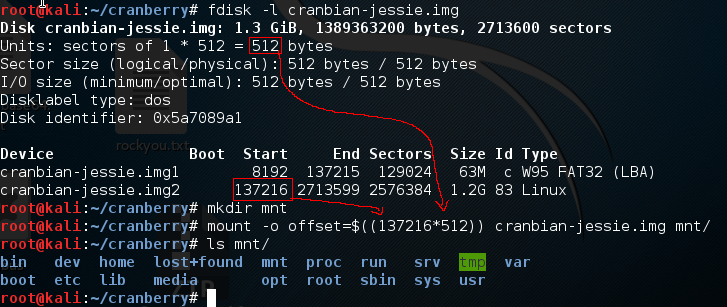
\includegraphics[width=\linewidth]{screenshots/cranbian_fdisk}
			\caption{The process of mounting the Cranbian image.}
			\label{fig.cranbian_fdisk}
		\end{figure}
		
		A comment on the red arrows in \autoref{fig.cranbian_fdisk}, $512$ is the size of each sector in the image and $137216$ is the start sector of the Linux file system. So with $137216 \times 512 = 70254592$ we have the offset needed to mount the image.\\
		\\
		Now that the image is mounted, it's time to put dear John to work. In \autoref{fig.cranbian_cracked} I do just that.

		\begin{figure}[H]
			\centering
			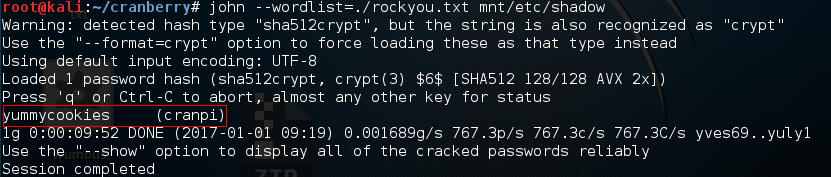
\includegraphics[width=\linewidth]{screenshots/cranbian_cracked}
			\caption{Cracking the shadow file. The password is 'yummycookies'}
			\label{fig.cranbian_cracked}
		\end{figure}
		
		So now we have the password for the user. Time to speak to Holly Everygreen and let her know what the password is.

		
	\subsection{How did you open each terminal door and where had the villain imprisoned Santa?}
		Alright, so there are five terminals scattered throughout the little world. Completing each terminal gives a password, which in turn allows access through the door next to the terminal.
		
		\subsubsection{Terminal 1: Elf House \#2} \label{terminal1}
			\begin{figure}[H]
				\centering
				\includegraphics[width=\linewidth]{"screenshots/terminals/Terminal 1 - First"}
			\end{figure}
			
			This is the screen that greets you when you open this terminal. So I guess we just have to read '/out.pcap,' easy peasy...
			\begin{figure}[H]
				\centering
				\includegraphics[scale=1]{"screenshots/terminals/Terminal 1 - ls pcap"}
			\end{figure}
			Except it seems that only \textit{itchy} can read the file, and I'm logged in as \textit{scratchy}. Trying to 'su itchy' prompts a password, which I don't have. ... What else, what else. Time to take a look at 'sudo,' more precisely 'sudo -l.'
			
			\begin{figure}[H]
				\centering
				\includegraphics[width=\linewidth]{"screenshots/terminals/Terminal 1 - sudo -l"}
			\end{figure}
			
			Alright, so there are a few commands available that I can run as \textit{itchy}. Time to run the first one and see if there's anything exciting.
			
			\begin{figure}[H]
				\centering
				\includegraphics[scale=1]{"screenshots/terminals/Terminal 1 - strings pcap"}
			\end{figure}
			\begin{figure}[H]
				\centering
				\includegraphics[width=\linewidth]{"screenshots/terminals/Terminal 1 - strings pcap pt3"}
			\end{figure}
			
			Browsing through the output of 'strings' does indeed show something exciting. The first red box shows the first part of the password, 'santasli', the second shows the GET request for what I believe to be the place to find the second half of the password.\\
			\\
			But first, I'll make a guess that the password is 'santaslittlehelper'.
			\begin{figure}[H]
				\centering
				\includegraphics[scale=1]{"screenshots/doors/Door code 1"}
			\end{figure}
		
			And lo and behold, it is the password.\\
			\\
			However, for completeness sake, it is time to try and find the second half of the password and as it turns out, the second half does not show in the 'strings' output.\\
			\\
			A few observations, before jumping the gun on 'tcpdump', it seems the GET requests where to \textit{/firsthalf.html} and \textit{/secondhalf.bin} and the marker for the first half of the password seems to be \textit{part1}, so an educated guess would be to search for \textit{part2} in the pcap.\\
			\\
			So with that in mind, it's time to run 'tcpdump' and pipe it into a grep to see if we can catch anything. 
			
			\begin{figure}[H]
				\centering
				\includegraphics[width=\linewidth]{"screenshots/terminals/Terminal 1 - tcpdump grep pt 1"}
			\end{figure}
			
			Well, it's a good start. It catches the first password. Now, since the theory is that the second part is embedded into the \textit{secondhalf.bin} file, the text might be separated by some obscure characters, so time to try another grep.
			
			\begin{figure}[H]
				\centering
				\includegraphics[width=\linewidth]{"screenshots/terminals/Terminal 1 - tcpdump grep pt 2"}
			\end{figure}
			
			Excellent, this time both parts of the password showed up, and it also confirmed the guess of 'santaslittlehelper.'
			
		
		
		
		\subsubsection{Terminal 2: The Workshop (Bottom)} \label{terminal2}
			\begin{figure}[H]
				\centering
				\includegraphics[width=\linewidth]{"screenshots/terminals/Terminal 2 - First"}
			\end{figure}
			
			Great. Stuff hidden somewhere, huh? I guess the first thing to do a little \textit{ls}'ing
			\begin{figure}[H]
				\centering
				\includegraphics[scale=1]{"screenshots/terminals/Terminal 2 - ls -al"}
			\end{figure}
			
			Would you look at that? There's a doormat, and everyone knows that you hide keys underneath doormats. Time to see if we can find any files in there, of if it's just a decoy.
			\begin{figure}[H]
				\centering
				\includegraphics[width=\linewidth]{"screenshots/terminals/Terminal 2 - find"}
			\end{figure}
			
			Uh, what? That looks like something that needs to be escaped at every step. And this terminal does \textbf{not} have tab-completion.
			
			\begin{figure}[H]
				\centering
				\includegraphics[width=\linewidth]{"screenshots/terminals/Terminal 2 - cd + cat"}
			\end{figure}
			
			Okay, a painstaking \textit{cd}'ing later and it is possible to \textit{cat} the file. Thus providing the key for the next door.



		\subsubsection{Terminal 3: The Workshop - Santa's Office } \label{terminal3}
			\begin{figure}[H]
				\centering
				\includegraphics[width=\linewidth]{"screenshots/terminals/Terminal 3 - First"}
			\end{figure}
			
			Hello, Joshua.

			\begin{figure}[H]
				\centering
				\includegraphics[width=\linewidth]{"screenshots/terminals/Terminal 3 - I dont understand"}
			\end{figure}
			
			Mkay. Or not. Well, turns out just 'Hello.' works. A bit of Google-foo and the full script is located\footnote{Located at \url{https://github.com/abs0/wargames/blob/master/wargames.sh}.}, however the script needed a little bit of modification.
			
			\begin{figure}[H]
				\centering
				\includegraphics[width=\linewidth]{"screenshots/terminals/Terminal 3 - First full"}
			\end{figure}
			\textit{Missing the side selection here, I choose '2'.}
			\begin{figure}[H]
				\centering
				\includegraphics[width=\linewidth]{"screenshots/terminals/Terminal 3 - Final"}
			\end{figure}
			
			And there we have it folks, the password for the next door.
			
			

		\subsubsection{Terminal 4: The Workshop (Top)} \label{terminal4}
			\begin{figure}[H]
				\centering
				\includegraphics[width=\linewidth]{"screenshots/terminals/Terminal 4 - First"}
			\end{figure}
			
			So a classic game of Hunt the Wumpus\footnote{Wiki page at \url{https://en.wikipedia.org/wiki/Hunt_the_Wumpus}}, now reversing stuff is in no form, way or shape my strong suit.\\
			\\
			So first things first, just play the game as it's meant to be played and that actually worked out perfectly fine. I completed the challenge in around 10 minutes time.\\
			\\
			However, for the sake of having fun and since I'm allowed to cheat, it's time to pull out the \textit{strings} command and take a look at what strings there are in the Wumpus binary.
			
			\begin{figure}[H]
				\centering
				\includegraphics[width=\linewidth]{"screenshots/terminals/Terminal 4 - ls"}
			\end{figure}
			\begin{figure}[H]
				\centering
				\includegraphics[width=\linewidth]{"screenshots/terminals/Terminal 4 - strings"}
			\end{figure}

			So straight away, this looks fishy. Is it possible to change the number of caves, bats etc., in the game? And what's that \textit{a:b:hp:r:t:} rubbish about? Let's keep going through the output.		
			
			\begin{figure}[H]
				\centering
				\includegraphics[width=\linewidth]{"screenshots/terminals/Terminal 4 - strings pt2"}
			\end{figure}

			So it seems as if there once were a file containing some sort of information about the game, but who knows.			
			
			\begin{figure}[H]
				\centering
				\includegraphics[width=\linewidth]{"screenshots/terminals/Terminal 4 - strings pt3"}
			\end{figure}
			
			Now, this confirms the suspicion about the game taking arguments of sorts. The arguments might be related to the odd string above.\\
			\\
			After searching google for "a:b:hp:r:t:" I found \textit{wumpus.c}\footnote{Located at \url{http://gentoo.osuosl.org/distfiles/wump.c}} and this file seems to let me know what the arguments are, and what they stand for.\\
			\begin{itemize}
				\item a - Amount of arrows the player can carry.
				\item b - Amount of bats in the game.
				\item h - Hard mode, no thanks.
				\item p - Amount of pits.
				\item r - Amount of rooms
				\item t - Amount of tunnels.		
			\end{itemize}
		
			So, with this information I'm ready to play the game.
			
			\begin{figure}[H]
				\centering
				\includegraphics[width=\linewidth]{"screenshots/terminals/Terminal 4 - wumpus run"}
			\end{figure}
			
			With a stroke of luck and the game is completed in the very first move.

		\subsubsection{Terminal 5: Train Station} \label{terminal5}
			\begin{figure}[H]
				\centering
				\includegraphics[width=\linewidth]{"screenshots/terminals/Terminal 5 - First"}
			\end{figure}
			
			Huh. So some sort of menu that we need to play around with.
			
			\begin{figure}[H]
				\centering
				\includegraphics[scale=1]{"screenshots/terminals/Terminal 5 - Start pt1"}
			\end{figure}
			
			So it seems that I need to find a password, to be able to start this thing.	
			
			\begin{figure}[H]
				\centering
				\includegraphics[scale=1]{"screenshots/terminals/Terminal 5 - Status"}
			\end{figure}
			
			Top speed 88mph and the flux capacitor is fluxing. Excellent. This better be time travel!
			
			\begin{figure}[H]
				\centering
				\includegraphics[width=\linewidth]{"screenshots/terminals/Terminal 5 - help screen"}
			\end{figure}
			
			So this is what is presented by the HELP command. Would you look at that, seems like there is a little hint for us. Now if this is showing the help file with \textit{less}, then typing ! and hitting enter should open a shell for us.
			
			\begin{figure}[H]
				\centering
				\includegraphics[width=\linewidth]{"screenshots/terminals/Terminal 5 - sh"}
			\end{figure}
			
			And there it is, the shell. And also the files that we need to look at. \textit{TrainHelper.txt} contains the help information, \textit{Train\_Console} contains the following
			
			\begin{figure}[H]
				\centering
				\includegraphics[width=\linewidth]{"screenshots/terminals/Terminal 5 - less Train_Console"}
			\end{figure}
			
			There's the password we need. However, maybe it's possible to run \textit{ActivateTrain} directly.
			
			\begin{figure}[H]
				\centering
				\includegraphics[width=\linewidth]{"screenshots/terminals/Terminal 5 - time travel"}
			\end{figure}
			
			Great success, it can be start with and without the password. So that's the last of the terminals down.
			
		
\end{document}